% Options for packages loaded elsewhere
\PassOptionsToPackage{unicode}{hyperref}
\PassOptionsToPackage{hyphens}{url}
\PassOptionsToPackage{dvipsnames,svgnames,x11names}{xcolor}
%
\documentclass[
  letterpaper,
  DIV=11,
  numbers=noendperiod]{scrartcl}

\usepackage{amsmath,amssymb}
\usepackage{lmodern}
\usepackage{iftex}
\ifPDFTeX
  \usepackage[T1]{fontenc}
  \usepackage[utf8]{inputenc}
  \usepackage{textcomp} % provide euro and other symbols
\else % if luatex or xetex
  \usepackage{unicode-math}
  \defaultfontfeatures{Scale=MatchLowercase}
  \defaultfontfeatures[\rmfamily]{Ligatures=TeX,Scale=1}
\fi
% Use upquote if available, for straight quotes in verbatim environments
\IfFileExists{upquote.sty}{\usepackage{upquote}}{}
\IfFileExists{microtype.sty}{% use microtype if available
  \usepackage[]{microtype}
  \UseMicrotypeSet[protrusion]{basicmath} % disable protrusion for tt fonts
}{}
\makeatletter
\@ifundefined{KOMAClassName}{% if non-KOMA class
  \IfFileExists{parskip.sty}{%
    \usepackage{parskip}
  }{% else
    \setlength{\parindent}{0pt}
    \setlength{\parskip}{6pt plus 2pt minus 1pt}}
}{% if KOMA class
  \KOMAoptions{parskip=half}}
\makeatother
\usepackage{xcolor}
\setlength{\emergencystretch}{3em} % prevent overfull lines
\setcounter{secnumdepth}{-\maxdimen} % remove section numbering
% Make \paragraph and \subparagraph free-standing
\ifx\paragraph\undefined\else
  \let\oldparagraph\paragraph
  \renewcommand{\paragraph}[1]{\oldparagraph{#1}\mbox{}}
\fi
\ifx\subparagraph\undefined\else
  \let\oldsubparagraph\subparagraph
  \renewcommand{\subparagraph}[1]{\oldsubparagraph{#1}\mbox{}}
\fi


\providecommand{\tightlist}{%
  \setlength{\itemsep}{0pt}\setlength{\parskip}{0pt}}\usepackage{longtable,booktabs,array}
\usepackage{calc} % for calculating minipage widths
% Correct order of tables after \paragraph or \subparagraph
\usepackage{etoolbox}
\makeatletter
\patchcmd\longtable{\par}{\if@noskipsec\mbox{}\fi\par}{}{}
\makeatother
% Allow footnotes in longtable head/foot
\IfFileExists{footnotehyper.sty}{\usepackage{footnotehyper}}{\usepackage{footnote}}
\makesavenoteenv{longtable}
\usepackage{graphicx}
\makeatletter
\def\maxwidth{\ifdim\Gin@nat@width>\linewidth\linewidth\else\Gin@nat@width\fi}
\def\maxheight{\ifdim\Gin@nat@height>\textheight\textheight\else\Gin@nat@height\fi}
\makeatother
% Scale images if necessary, so that they will not overflow the page
% margins by default, and it is still possible to overwrite the defaults
% using explicit options in \includegraphics[width, height, ...]{}
\setkeys{Gin}{width=\maxwidth,height=\maxheight,keepaspectratio}
% Set default figure placement to htbp
\makeatletter
\def\fps@figure{htbp}
\makeatother

\KOMAoption{captions}{tableheading}
\makeatletter
\makeatother
\makeatletter
\makeatother
\makeatletter
\@ifpackageloaded{caption}{}{\usepackage{caption}}
\AtBeginDocument{%
\ifdefined\contentsname
  \renewcommand*\contentsname{Table of contents}
\else
  \newcommand\contentsname{Table of contents}
\fi
\ifdefined\listfigurename
  \renewcommand*\listfigurename{List of Figures}
\else
  \newcommand\listfigurename{List of Figures}
\fi
\ifdefined\listtablename
  \renewcommand*\listtablename{List of Tables}
\else
  \newcommand\listtablename{List of Tables}
\fi
\ifdefined\figurename
  \renewcommand*\figurename{Figure}
\else
  \newcommand\figurename{Figure}
\fi
\ifdefined\tablename
  \renewcommand*\tablename{Table}
\else
  \newcommand\tablename{Table}
\fi
}
\@ifpackageloaded{float}{}{\usepackage{float}}
\floatstyle{ruled}
\@ifundefined{c@chapter}{\newfloat{codelisting}{h}{lop}}{\newfloat{codelisting}{h}{lop}[chapter]}
\floatname{codelisting}{Listing}
\newcommand*\listoflistings{\listof{codelisting}{List of Listings}}
\makeatother
\makeatletter
\@ifpackageloaded{caption}{}{\usepackage{caption}}
\@ifpackageloaded{subcaption}{}{\usepackage{subcaption}}
\makeatother
\makeatletter
\@ifpackageloaded{tcolorbox}{}{\usepackage[many]{tcolorbox}}
\makeatother
\makeatletter
\@ifundefined{shadecolor}{\definecolor{shadecolor}{rgb}{.97, .97, .97}}
\makeatother
\makeatletter
\makeatother
\ifLuaTeX
  \usepackage{selnolig}  % disable illegal ligatures
\fi
\IfFileExists{bookmark.sty}{\usepackage{bookmark}}{\usepackage{hyperref}}
\IfFileExists{xurl.sty}{\usepackage{xurl}}{} % add URL line breaks if available
\urlstyle{same} % disable monospaced font for URLs
\hypersetup{
  pdftitle={Git Training},
  pdfauthor={Ross Dahlke},
  colorlinks=true,
  linkcolor={blue},
  filecolor={Maroon},
  citecolor={Blue},
  urlcolor={Blue},
  pdfcreator={LaTeX via pandoc}}

\title{Git Training}
\author{Ross Dahlke}
\date{}

\begin{document}
\maketitle
\ifdefined\Shaded\renewenvironment{Shaded}{\begin{tcolorbox}[boxrule=0pt, interior hidden, enhanced, frame hidden, breakable, sharp corners, borderline west={3pt}{0pt}{shadecolor}]}{\end{tcolorbox}}\fi

\renewcommand*\contentsname{Table of contents}
{
\hypersetup{linkcolor=}
\setcounter{tocdepth}{3}
\tableofcontents
}
\hypertarget{intro-to-git-training}{%
\section{Intro to Git Training}\label{intro-to-git-training}}

Welcome to Git training! Git is one of the most powerful and useful
programming fundamentals. However, it is seldom taught in school,
especially as a part of a social science research programs. In this
document, I hope to get you started on your own Git journey. This
document will certainly not cover everything related to Git but just a
few commands can provide \textbf{a lot} of value. When starting out, I
found it most useful to use it alongside a tutorial until I really felt
comfortable with it. I hope that this document can be that tutorial for
you.

\hypertarget{why-git}{%
\subsection{Why Git?}\label{why-git}}

Git is a version control system that makes programming faster, more
collaborative, and improves data integrity. The big idea is that you can
periodically save your code in a certain spot so that you, or a
collaborator, can easy track changes and restore older versions. It also
allows you get experimental. If you want to try out a crazy idea but you
don't want to mess up the existing code, no problem! That's what Git is
here for.

Git is all about connecting versions of code that are stored in the
central repository (let's just call it the cloud) and your local
computer.

If you want another explanation of Git, my programmer friends who are
way smarter than me swear by the video
\href{https://www.youtube.com/watch?v=1ffBJ4sVUb4\&ab_channel=HackersOnBoard}{Git
for Ages 4 And Up}

\hypertarget{git-clients}{%
\subsubsection{Git Clients}\label{git-clients}}

There are a variety of Git ``clients'' out there, including GitHub,
GitKraken, Bitbucket, etc. In this tutorial, I will be showing how to
use GitHub with the \emph{command line}. GitHub does have a
\href{https://desktop.github.com/}{desktop application} which can
abstract the use of the command line, but I personally prefer being a
little bit more ``hands-on'' to what is happening under the hood. If
there's interest, I'm happy to create a tutorial using the GitHub
Desktop app. Other Git storage systems, for example, Bitbucket, can be
used similarly this tutorial.

\hypertarget{github}{%
\subsection{GitHub}\label{github}}

\hypertarget{starting-with-github}{%
\subsubsection{Starting with GitHub}\label{starting-with-github}}

\begin{enumerate}
\def\labelenumi{\arabic{enumi}.}
\tightlist
\item
  Create a \href{https://github.com/}{GitHub} account
\item
  Configure your
  \href{https://docs.github.com/en/authentication/connecting-to-github-with-ssh/adding-a-new-ssh-key-to-your-github-account}{SSH
  key}

  \begin{enumerate}
  \def\labelenumii{\arabic{enumii}.}
  \item
    Open your terminal and check to see if you already have an SSH key
    using the command \texttt{ssh-add\ -l}
  \item
    If you do not, use the command

\begin{verbatim}
ssh-keygen -t ed25519 -C "your_email@example.com"
\end{verbatim}
  \item
    Press enter to use the default location
  \item
    Enter secure passphrase (or click enter for none)
  \item
    Use the command \texttt{cat\ .ssh/id\_ed25519.pub} to show your
    public key
  \item
    Copy that key to your clipboard
  \item
    Log into GitHub
  \item
    Click on settings

    \begin{figure}

    {\centering 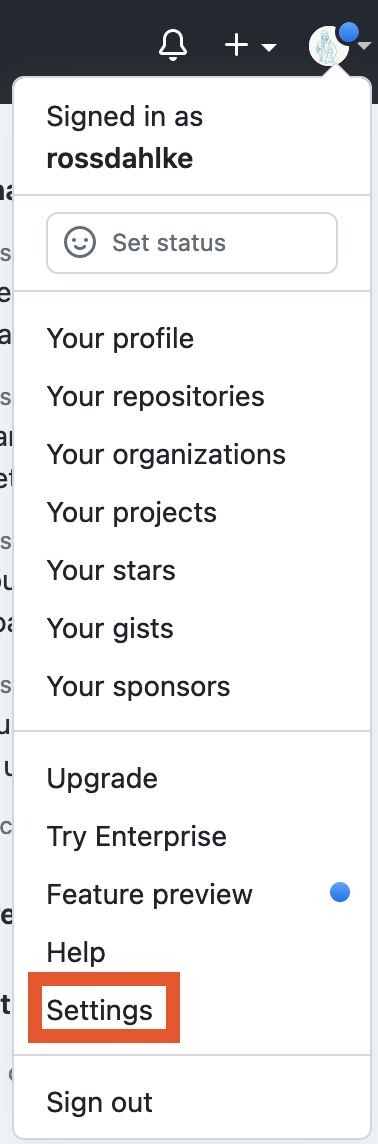
\includegraphics[width=0.3\textwidth,height=\textheight]{/images/settings.png}

    }

    \caption{settings}

    \end{figure}
  \item
    Select SSH and GPG keys

    \begin{figure}

    {\centering 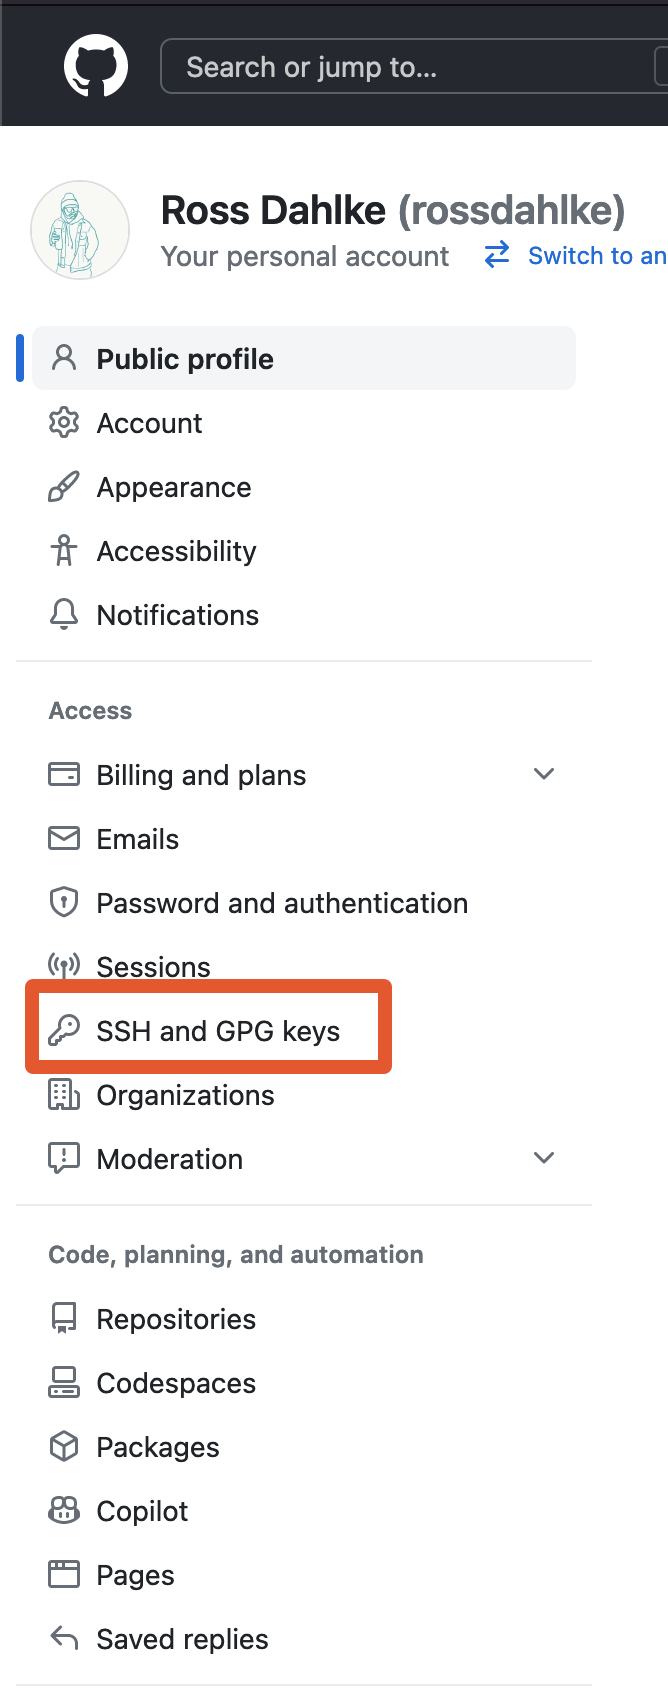
\includegraphics[width=0.4\textwidth,height=\textheight]{/images/ssh keys.png}

    }

    \caption{ssh keys button}

    \end{figure}
  \item
    Click New SSH Key

    \begin{figure}

    {\centering 
\includegraphics{/images/new ssh key.png}

    }

    \caption{new ssh key}

    \end{figure}
  \item
    Give your key a title

    \begin{figure}

    {\centering 
\includegraphics{/images/new ssh key.png}

    }

    \caption{ssh fields}

    \end{figure}
  \item
    Paste your public key into the Key field
  \item
    Click Add SSH Key
  \end{enumerate}
\end{enumerate}

\hypertarget{creating-a-new-repository}{%
\subsubsection{Creating a new
repository}\label{creating-a-new-repository}}

\begin{enumerate}
\def\labelenumi{\arabic{enumi}.}
\item
  Go to your GitHub \href{https://github.com/}{homepage}
\item
  On the left menu ``Top Repositories'' click the ``New'' button

  \begin{figure}

  {\centering 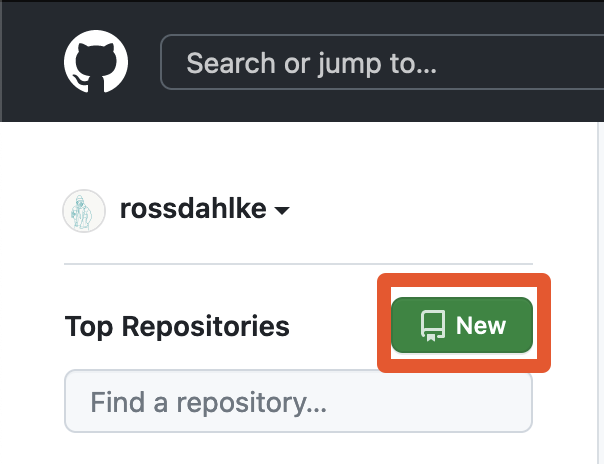
\includegraphics[width=0.5\textwidth,height=\textheight]{/images/new_repo.png}

  }

  \caption{Create a new repository}

  \end{figure}
\item
  Give your repository a name and fill out the remaining details
\item
  Congratulations, you just made a new repository! Right now, the
  repository only exists in the cloud.
\end{enumerate}

\hypertarget{downloading-a-repository}{%
\subsubsection{Downloading a
repository}\label{downloading-a-repository}}

\begin{enumerate}
\def\labelenumi{\arabic{enumi}.}
\item
  Go to the GitHub page of your repository (e.g.,
  \url{github.com/rossdahlke/git-training})
\item
  If you do not have the repository downloaded on your local computer,
  click on the ``Code'' dropdown

  \begin{figure}

  {\centering 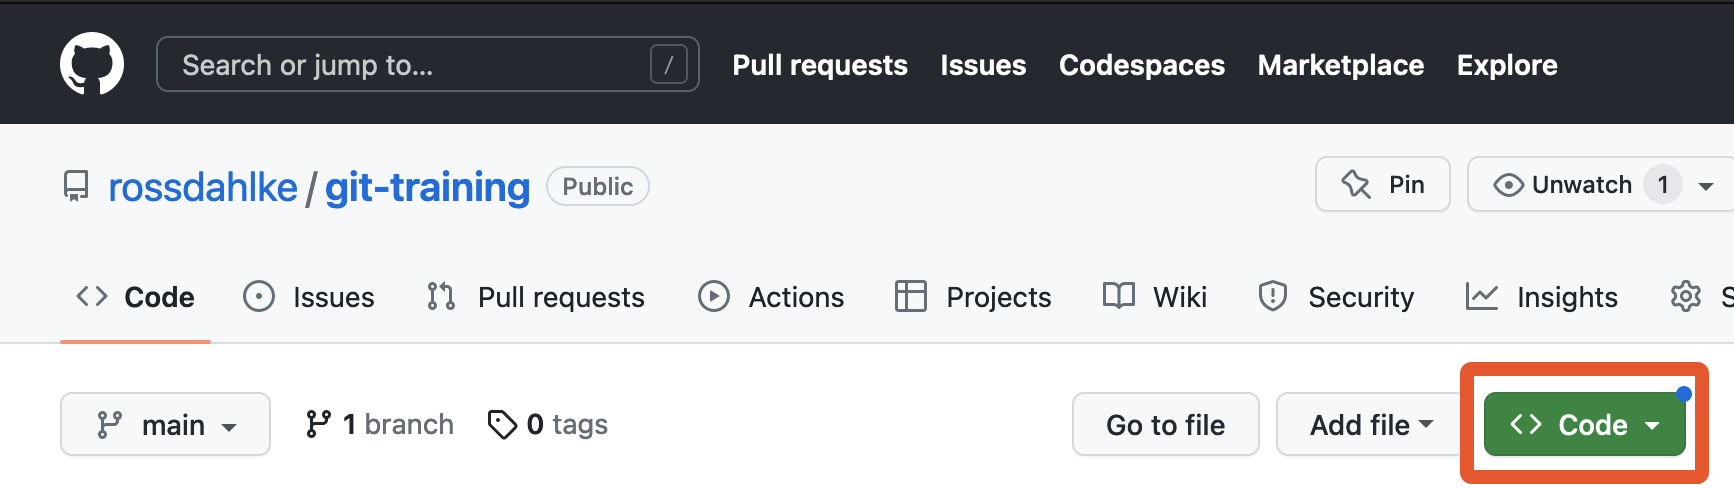
\includegraphics{/images/code_button.png}

  }

  \caption{Code Button}

  \end{figure}
\item
  Click on ``SSH'' and copy the git address (e.g.,
  ``git@github.com:rossdahlke/git-training.git'')

  \begin{figure}

  {\centering 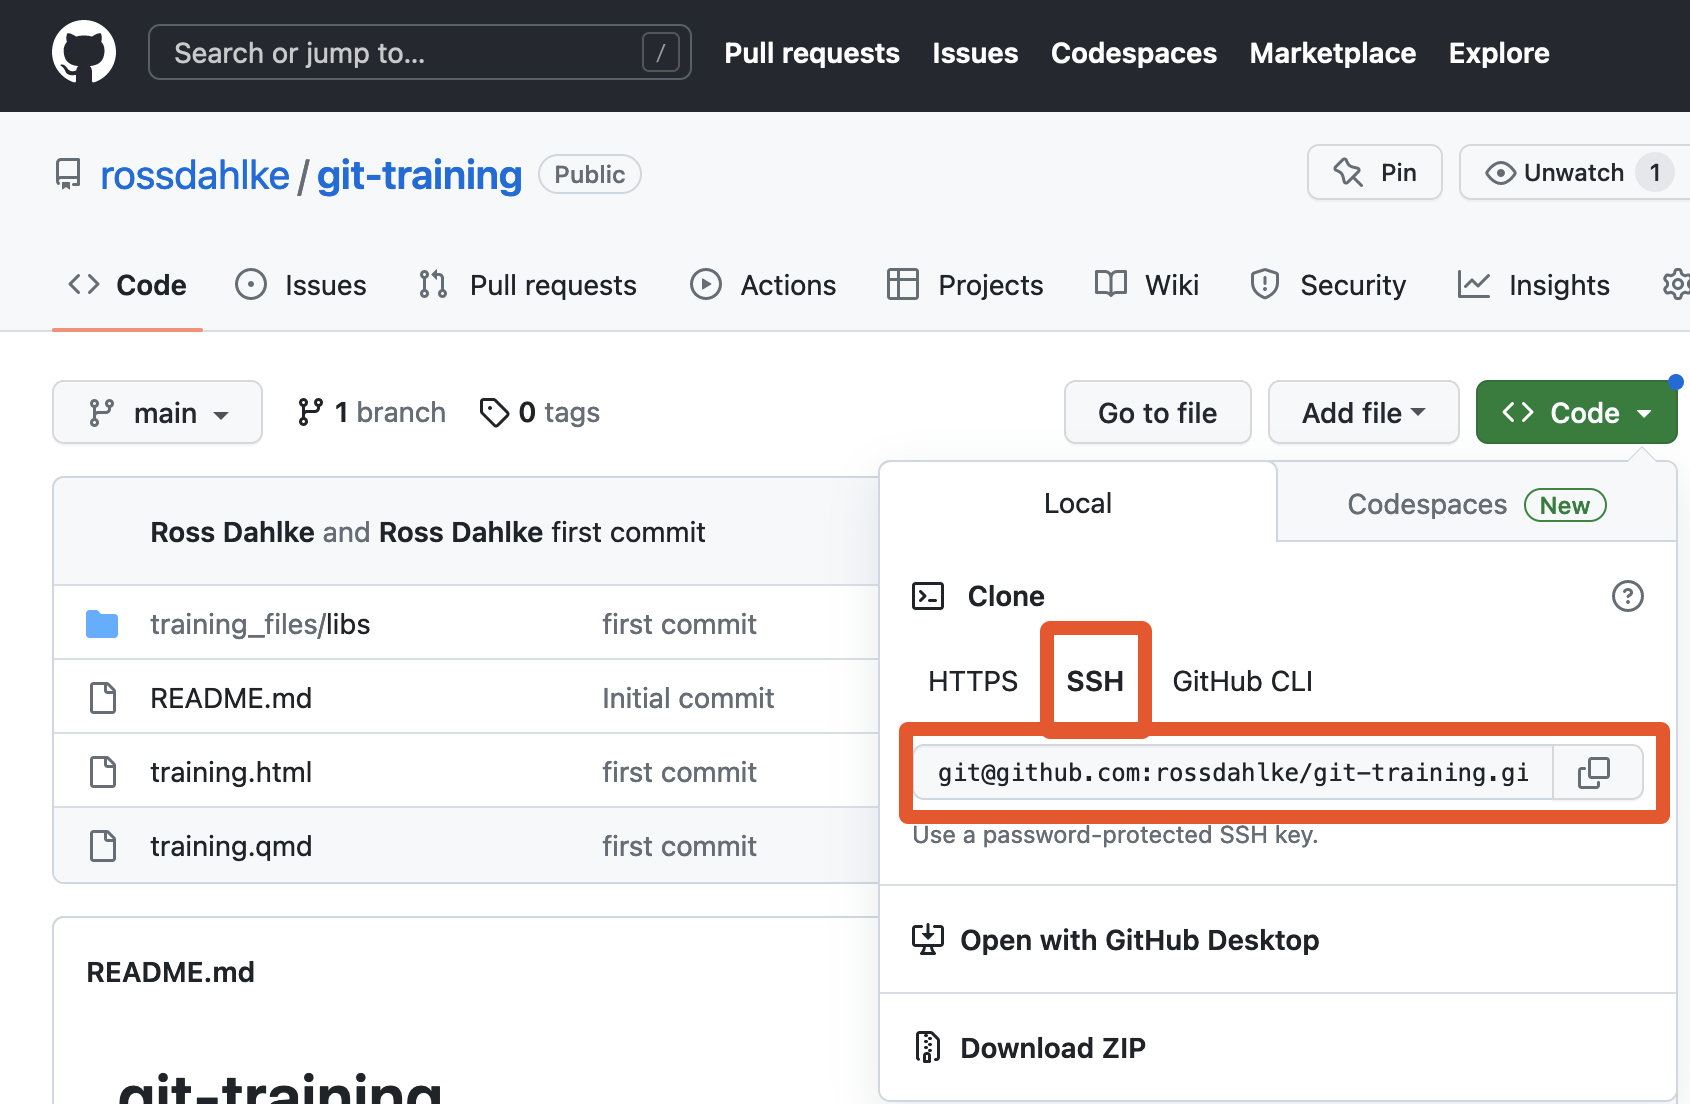
\includegraphics{/images/ssh.png}

  }

  \caption{ssh}

  \end{figure}
\item
  Open your terminal on your local computer or IDE
\item
  Use \texttt{ls} and \texttt{cd} to navigate to the folder that you
  want the repository to live in
\item
  In the terminal use the \texttt{git\ clone} function to ``clone'' the
  repository down to your local machine

  \begin{enumerate}
  \def\labelenumii{\arabic{enumii}.}
  \tightlist
  \item
    e.g.,
    \texttt{git\ clone\ git@github.com:rossdahlke/git-training.git}
  \end{enumerate}
\item
  Now, that repository should exist on your local computer
\item
  Make any changes you want your want to the code
\end{enumerate}

\hypertarget{sending-a-repository-back-up}{%
\subsubsection{Sending a repository back
up}\label{sending-a-repository-back-up}}

\begin{enumerate}
\def\labelenumi{\arabic{enumi}.}
\tightlist
\item
  Once you've made the changes you want to the file, you can ``commit''
  and ``push'' those changes back up to GitHub
\item
  Open your terminal on your local computer or use the terminal in your
  IDE
\item
  Use \texttt{ls} and \texttt{cd} to navigate to your Git repository
\item
  Check on the status of the files in your repository using the
  \texttt{git\ status} command

  \begin{enumerate}
  \def\labelenumii{\arabic{enumii}.}
  \tightlist
  \item
    Files in red are new/ edited files that are currently untracked
  \item
    Files in green are new/ edited files that are being tracked
  \end{enumerate}
\item
  Add the files you wish to ``commit'' up using the \texttt{git\ add}
  function

  \begin{enumerate}
  \def\labelenumii{\arabic{enumii}.}
  \tightlist
  \item
    e.g., \texttt{git\ add\ training.html}
  \end{enumerate}
\item
  You can check on the status of your files again using
  \texttt{git\ status}, notice that the files you just added should be
  green now
\item
  Commit the changes you made using the \texttt{git\ commit\ -m} command
  followed by a message in quotes (e.g.,
  \texttt{git\ commit\ -m\ "first\ commit"})
\item
  Push your changes back to GitHub using the \texttt{git\ push} command
\item
  Check on GitHub to make sure your changes are there
\item
  Now, other people can go and \texttt{git\ clone} your files and push
  them back
\end{enumerate}

\textbf{Just remember the steps of ``add, commit, push''!}

\hypertarget{getting-updates-to-a-repository-that-someone-else-pushed}{%
\subsubsection{Getting updates to a repository that someone else
pushed}\label{getting-updates-to-a-repository-that-someone-else-pushed}}

\begin{enumerate}
\def\labelenumi{\arabic{enumi}.}
\tightlist
\item
  If you already have a repository cloned onto your local computer and
  want to get the latest version of the repo (i.e., after someone else
  pushed up their changes) use the \texttt{git\ pull} command
\end{enumerate}



\end{document}
